\documentclass[tikz,border=20pt]{standalone}
\usepackage{amsmath,amssymb}
\usepackage{tikz}
\usetikzlibrary{matrix, arrows.meta, positioning, fit, backgrounds, calc}

\newcommand{\ideal}[1]{\langle #1\rangle}
\newcommand{\F}{\mathbb F}
\begin{document}
	
	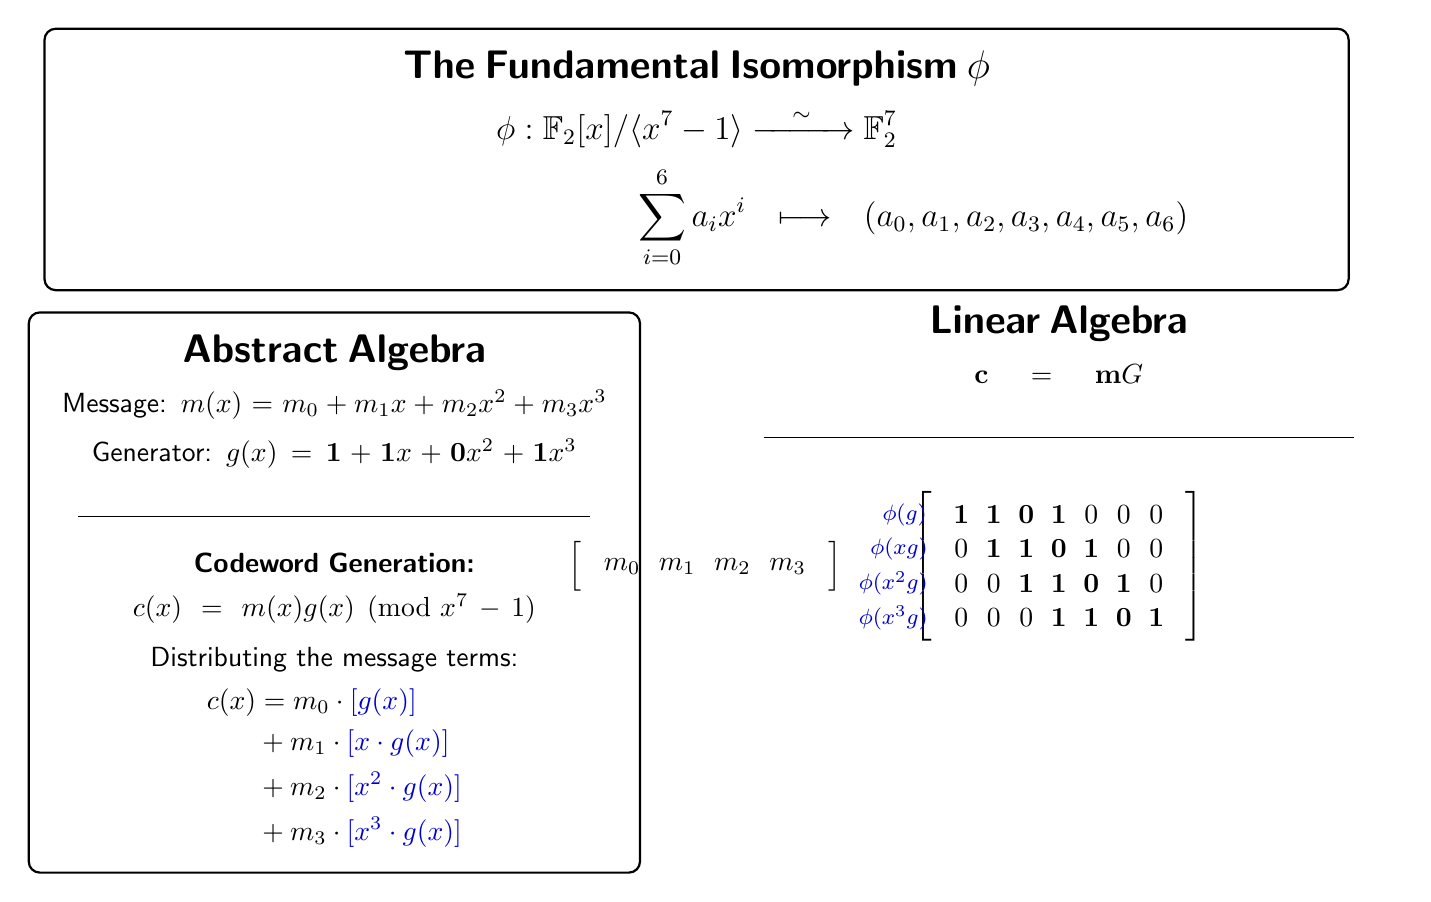
\begin{tikzpicture}[
		>=Latex,
		font=\sffamily,
		box/.style={draw, rounded corners, thick, align=center, fill=white, inner sep=8pt},
		highlight/.style={fill=red!15, rounded corners, inner sep=2pt},
		shiftbox/.style={draw=blue!60!black, thick, rounded corners, fill=blue!5, inner sep=6pt}
		]
		
		% =========================================================
		% 1. The Core Isomorphism Map
		% =========================================================
		\node[box, text width=16cm] (Iso) at (0, 4) {
			\centering\textbf{\Large The Fundamental Isomorphism $\phi$}\\[8pt]
			\large
			$\displaystyle \phi: \mathbb{F}_2[x]/\langle x^7-1 \rangle \xrightarrow{\quad\sim\quad} \mathbb{F}_2^7$\\[6pt]
			\hspace{5.5cm}$\displaystyle \sum_{i=0}^{6}a_ix^i \longmapsto (a_0, a_1, a_2, a_3, a_4, a_5, a_6)$
		};
		
		% =========================================================
		% 2. Polynomial View (Left Side)
		% =========================================================
		\node[box, text width=7.2cm, minimum height=6.5cm] (PolyBox) at (-4.6, -1.5) {
			\textbf{\Large Abstract Algebra}\\[6pt]
			Message: $m(x) = m_0 + m_1x + m_2x^2 + m_3x^3$\\[6pt]
			Generator: $g(x) = \mathbf{1} + \mathbf{1}x + \mathbf{0}x^2 + \mathbf{1}x^3$\\[8pt]
			\rule{6.5cm}{0.5pt}\\[8pt]
			\textbf{Codeword Generation:}\\[4pt]
			$c(x) = m(x)g(x) \pmod{x^7-1}$\\[6pt]
			Distributing the message terms:\\[4pt]
			$\begin{aligned}
				c(x) &= m_0 \cdot \textcolor{blue!80!black}{[g(x)]} \\
				&+ m_1 \cdot \textcolor{blue!80!black}{[x \cdot g(x)]} \\
				&+ m_2 \cdot \textcolor{blue!80!black}{[x^2 \cdot g(x)]} \\
				&+ m_3 \cdot \textcolor{blue!80!black}{[x^3 \cdot g(x)]}
			\end{aligned}$
		};
		
		% =========================================================
		% 3. Linear Algebra View (Right Side)
		% =========================================================
		% Instead of a nested tikzpicture, we group elements in a scope 
		% and track their bounding box to draw the panel behind them later.
		\begin{scope}[local bounding box=MatrixContents]
			
			\node[text width=8.5cm, align=center] (LinAlgTitle) at (4.6, 1.3) {
				\textbf{\Large Linear Algebra}\\[6pt]
				$\mathbf{c} = \mathbf{m} G$\\[8pt]
				\rule{7.5cm}{0.5pt}
			};
			
			\matrix (M) [matrix of math nodes, left delimiter={[}, right delimiter={]}, below=0.5cm of LinAlgTitle, nodes={inner sep=3pt, anchor=center}] {
				\mathbf{1} & \mathbf{1} & \mathbf{0} & \mathbf{1} & 0 & 0 & 0 \\
				0 & \mathbf{1} & \mathbf{1} & \mathbf{0} & \mathbf{1} & 0 & 0 \\
				0 & 0 & \mathbf{1} & \mathbf{1} & \mathbf{0} & \mathbf{1} & 0 \\
				0 & 0 & 0 & \mathbf{1} & \mathbf{1} & \mathbf{0} & \mathbf{1} \\
			};
			
			% Row labels
			\node[left=0.1cm of M-1-1, text=blue!80!black, font=\footnotesize] {$\phi(g)$};
			\node[left=0.1cm of M-2-1, text=blue!80!black, font=\footnotesize] {$\phi(xg)$};
			\node[left=0.1cm of M-3-1, text=blue!80!black, font=\footnotesize] {$\phi(x^2g)$};
			\node[left=0.1cm of M-4-1, text=blue!80!black, font=\footnotesize] {$\phi(x^3g)$};
			
			% Vector m
			\matrix (mVec) [matrix of math nodes, left delimiter={[}, right delimiter={]}, left=1.4cm of M] {
				m_0 & m_1 & m_2 & m_3 \\
			};
			
		\end{scope}
		
%		% Draw the background box and the blue highlight strips using the backgrounds library
%		\begin{scope}[on background layer]
%			% Outer Red Panel
%			\node[box, fill=red!4, draw=red!60!black, fit=(MatrixContents), minimum height=6.5cm, inner sep=10pt] (RealMatrixBox) {};
%			
%			% Shift boxes inside the matrix
%			\node[fill=blue!10, rounded corners, fit=(M-1-1)(M-1-4)] {};
%			\node[fill=blue!10, rounded corners, fit=(M-2-2)(M-2-5)] {};
%			\node[fill=blue!10, rounded corners, fit=(M-3-3)(M-3-6)] {};
%			\node[fill=blue!10, rounded corners, fit=(M-4-4)(M-4-7)] {};
%		\end{scope}
%		
%		% =========================================================
%		% 4. Equivalence Connectors
%		% =========================================================
%		\draw[<->, ultra thick, dashed, gray!60!black] (PolyBox.east) -- (RealMatrixBox.west) 
%		node[midway, above, font=\bfseries] {$\phi$}
%		node[midway, below, align=center, font=\footnotesize] {Multiplication \\ $\Updownarrow$ \\ Linear Combo};
%		
%		% =========================================================
%		% 5. The Cyclic Shift Wrap-around (Bottom Box)
%		% =========================================================
%		\node[box, text width=16cm, fill=blue!5, draw=blue!60!black] (Cyclic) at (0, -6.0) {
%			\centering\textbf{\Large What makes it "Cyclic"?}\\[8pt]
%			\large
%			If we multiplied by $x^4$, we would get $x^4 \cdot g(x) = x^4 + x^5 + x^7$. \\
%			But in our ring, $x^7 \equiv 1$. Therefore $x^4 \cdot g(x) \equiv \mathbf{1} + x^4 + x^5$.\\[6pt]
%			In the vector space, this is a cyclic wrap-around: $\mathbf{\phi(x^4g)} = (\mathbf{1}, 0, 0, 0, 1, 1, 0)$.\\[6pt]
%			\textit{The ideal $\langle g(x) \rangle$ is exactly the row-space of $G$, closed under this wrap-around shift.}
%		};
%		
%		% Connections to the bottom box
%		\draw[->, thick, gray!60, rounded corners] (RealMatrixBox.south) |- ($(Cyclic.north)+(0,0.5)$) -- (Cyclic.north);
%		\draw[->, thick, gray!60, rounded corners] (PolyBox.south) |- ($(Cyclic.north)+(0,0.5)$) -- (Cyclic.north);
	\end{tikzpicture}


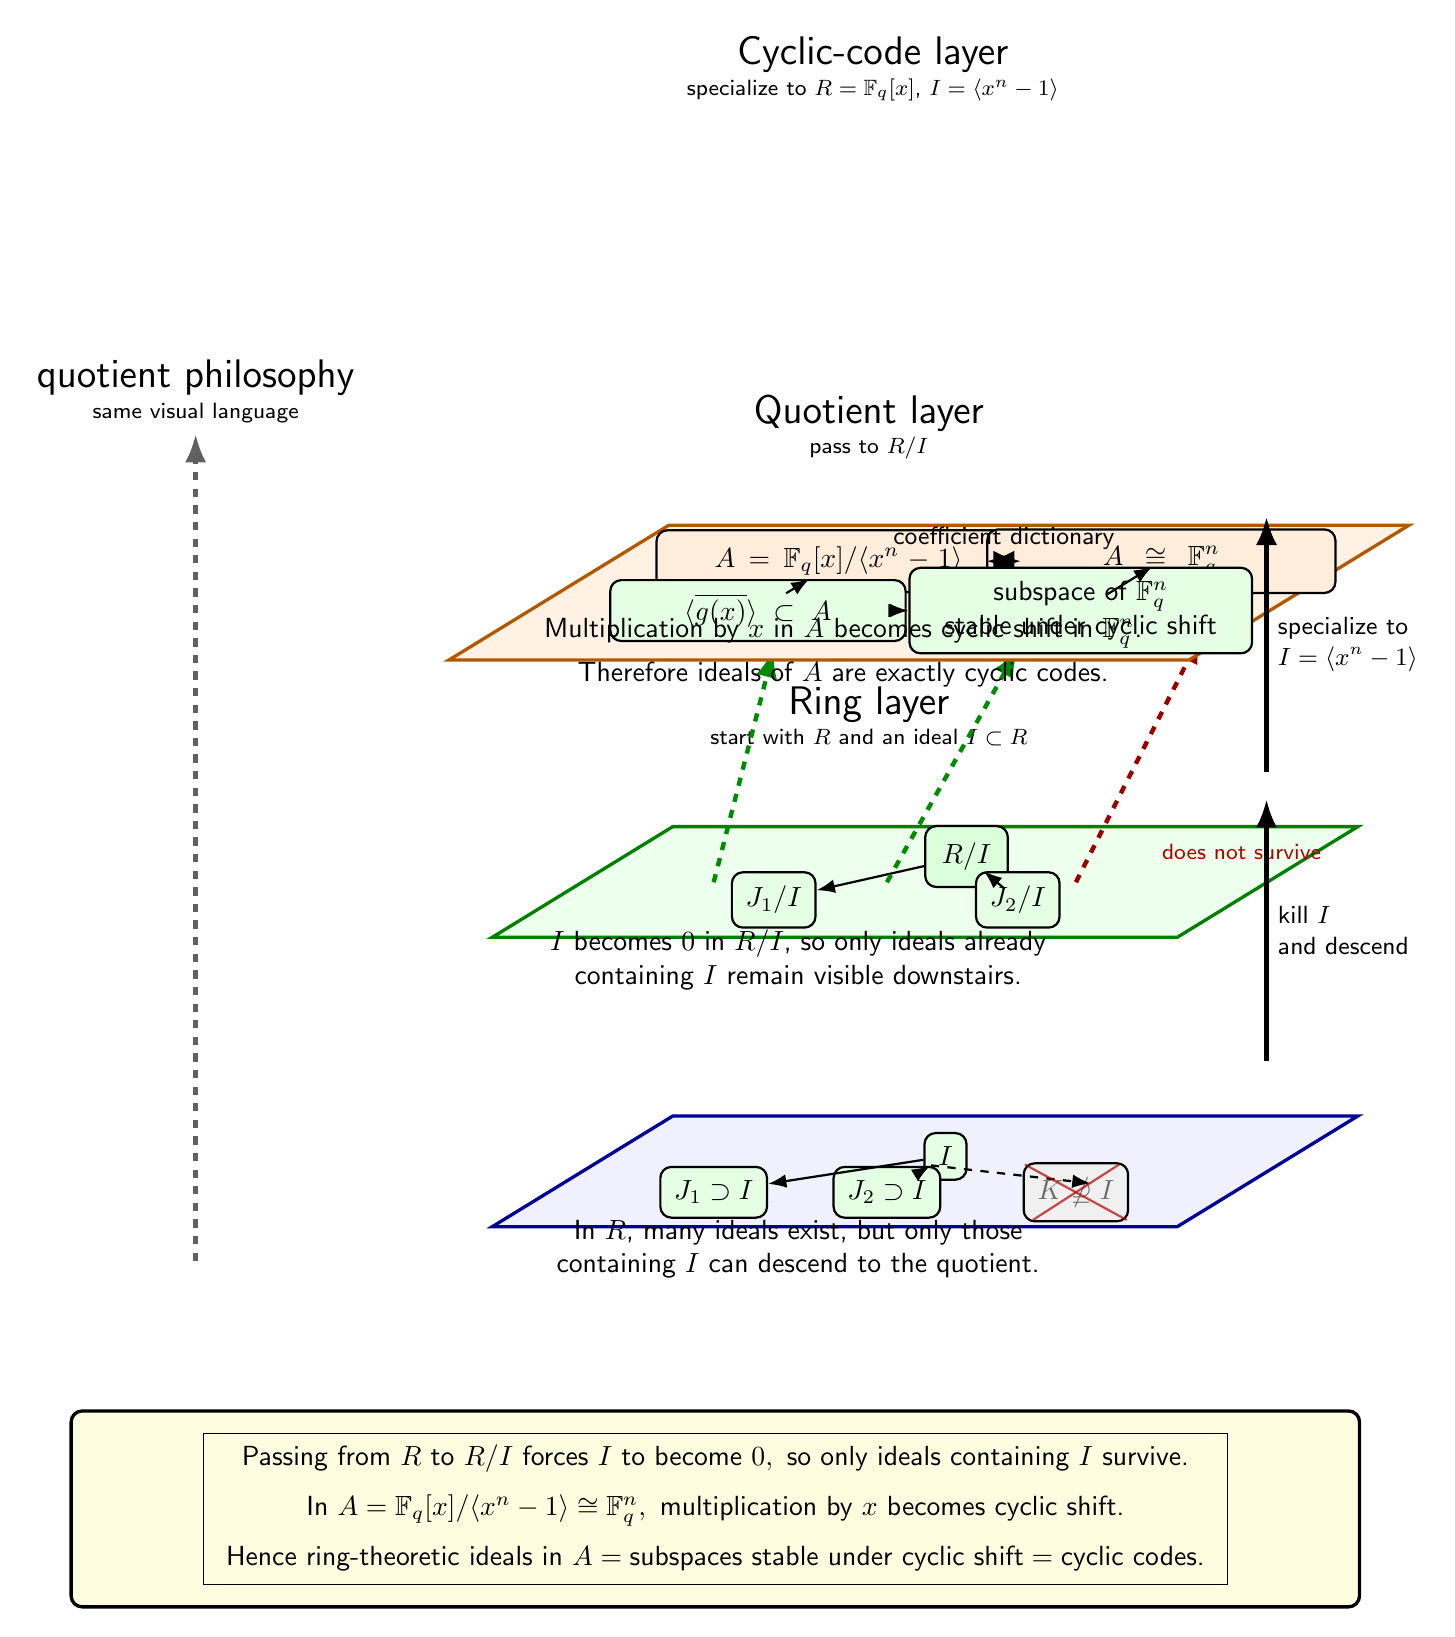
\begin{tikzpicture}[
	x={(1cm,0cm)},
	y={(0.62cm,0.38cm)},
	z={(0cm,1.75cm)},
	scale=1.0,
	font=\sffamily,
	>=Latex,
	good/.style={draw, rounded corners, thick, fill=green!10, align=center, inner sep=5pt},
	bad/.style={draw, rounded corners, thick, fill=gray!12, text opacity=0.55, align=center, inner sep=5pt},
	bigpanel/.style={draw, rounded corners, very thick, inner sep=8pt},
	ringpanel/.style={bigpanel, fill=blue!6, draw=blue!60!black},
	quopanel/.style={bigpanel, fill=green!7, draw=green!50!black},
	codepanel/.style={bigpanel, fill=orange!10, draw=orange!70!black},
	sumbox/.style={draw, rounded corners, very thick, fill=yellow!12, align=center, inner sep=8pt}
	]
	
	% --------------------------------------------------
	% Global vertical guide
	% --------------------------------------------------
	\draw[->, ultra thick, dashed, gray!75!black]
	(-5.2,0,-0.4) -- (-5.2,0,5.6)
	node[above, align=center, text=black]
	{\Large quotient philosophy\\[-1pt]\footnotesize same visual language};
	
	% ==================================================
	% Layer 1: Ring R
	% ==================================================
	\begin{scope}[shift={(0,0,0)}]
		
		\draw[fill=blue!6, draw=blue!60!black, very thick]
		(-1.0,-0.7) -- (7.7,-0.7) -- (7.7,3.0) -- (-1.0,3.0) -- cycle;
		
		\node[align=center] at (3.35,0,3.55)
		{\Large Ring layer\\[-1pt]\footnotesize start with $R$ and an ideal $I\subset R$};
		
		\node[good] (I) at (3.3,1.65) {$I$};
		
		\node[good] (J1) at (1.1,0.45) {$J_1\supset I$};
		\node[good] (J2) at (3.3,0.45) {$J_2\supset I$};
		\node[bad]  (K)  at (5.7,0.45) {$K\nsupseteq I$};
		
		\draw[->, thick] (I) -- (J1);
		\draw[->, thick] (I) -- (J2);
		\draw[->, thick, dashed] (3.3,1.35) -- (5.7,0.75);
		
		\draw[thick, red!70!black, opacity=0.7] ($(K.north west)+(0.08,-0.08)$) -- ($(K.south east)+(-0.08,0.08)$);
		\draw[thick, red!70!black, opacity=0.7] ($(K.south west)+(0.08,0.08)$) -- ($(K.north east)+(-0.08,-0.08)$);
		
		\node[align=center, text width=7.0cm] at (3.35,-1.45)
		{In $R$, many ideals exist, but only those containing $I$ can descend to the quotient.};
		
	\end{scope}
	
	% ==================================================
	% Layer 2: Quotient R/I
	% ==================================================
	\begin{scope}[shift={(0,0,2.1)}]
		
		\draw[fill=green!7, draw=green!50!black, very thick]
		(-1.0,-0.7) -- (7.7,-0.7) -- (7.7,3.0) -- (-1.0,3.0) -- cycle;
		
		\node[align=center] at (3.35,0,3.55)
		{\Large Quotient layer\\[-1pt]\footnotesize pass to $R/I$};
		
		\node[draw, rounded corners, thick, fill=green!14, align=center, inner sep=6pt]
		(Q) at (3.35,2.0) {$R/I$};
		
		\node[good] (QJ1) at (1.8,0.55) {$J_1/I$};
		\node[good] (QJ2) at (4.9,0.55) {$J_2/I$};
		
		\draw[->, thick] (Q) -- (QJ1);
		\draw[->, thick] (Q) -- (QJ2);
		
		% vertical survival arrows
		\draw[->, ultra thick, dashed, green!55!black] (1.1,0.45,0.15) -- (1.8,0.55,1.82);
		\draw[->, ultra thick, dashed, green!55!black] (3.3,0.45,0.15) -- (4.9,0.55,1.82);
		
		% K dies
		\draw[->, ultra thick, dashed, red!60!black] (5.7,0.45,0.15) -- (6.45,1.8,1.65);
		\node[align=center, text=red!70!black] at (6.75,2.15)
		{\footnotesize does not survive};
		
		\node[align=center, text width=7.2cm] at (3.35,-1.45)
		{$I$ becomes $0$ in $R/I$, so only ideals already containing $I$ remain visible downstairs.};
		
	\end{scope}
	
	% ==================================================
	% Layer 3: Cyclic-code specialization
	% ==================================================
	\begin{scope}[shift={(0,0,4.2)}]
		
		\draw[fill=orange!10, draw=orange!70!black, very thick]
		(-1.3,-1.1) -- (8.1,-1.1) -- (8.1,3.4) -- (-1.3,3.4) -- cycle;
		
		\node[align=center] at (3.4,0,4.05)
		{\Large Cyclic-code layer\\[-1pt]\footnotesize specialize to $R=\F_q[x]$, $I=\ideal{x^n-1}$};
		
		\node[draw, rounded corners, thick, fill=orange!14, align=center, inner sep=6pt, text width=4.2cm]
		(A) at (1.6,2.2) {$\displaystyle A=\F_q[x]/\ideal{x^n-1}$};
		
		\node[draw, rounded corners, thick, fill=orange!14, align=center, inner sep=6pt, text width=4.0cm]
		(V) at (5.7,2.2) {$\displaystyle A\cong \F_q^n$};
		
		\draw[<->, ultra thick] (A) -- node[above] {\small coefficient dictionary} (V);
		
		\node[good, text width=3.4cm] (poly) at (1.6,0.55)
		{$\langle \overline{g(x)}\rangle \subset A$};
		
		\node[good, text width=4.0cm] (vec) at (5.7,0.55)
		{subspace of $\F_q^n$\\stable under cyclic shift};
		
		\draw[->, thick] (A) -- (poly);
		\draw[->, thick] (V) -- (vec);
		\draw[<->, thick, dashed] (poly) -- (vec);
		
		\node[align=center, text width=7.6cm] at (3.55,-0.85)
		{Multiplication by $x$ in $A$ becomes cyclic shift in $\F_q^n$.\\[4pt]
			Therefore ideals of $A$ are exactly cyclic codes.};
		
	\end{scope}
	
	% ==================================================
	% Connecting arrows between layers
	% ==================================================
	\draw[->, ultra thick] (8.4,0,1.05) -- (8.4,0,2.95)
	node[midway, right, align=left] {\small kill $I$\\[-1pt]\small and descend};
	
	\draw[->, ultra thick] (8.4,0,3.15) -- (8.4,0,5.0)
	node[midway, right, align=left] {\small specialize to\\[-1pt]\small $I=\ideal{x^n-1}$};
	
	% ==================================================
	% Bottom summary
	% ==================================================
	\node[sumbox, text width=15.8cm] at (1.4,0,-2.2)
	{$\displaystyle
		\boxed{
			\begin{array}{c}
				\text{Passing from }R\text{ to }R/I\text{ forces }I\text{ to become }0,
				\text{ so only ideals containing }I\text{ survive.}
				\\[6pt]
				\text{In }A=\F_q[x]/\ideal{x^n-1}\cong \F_q^n,
				\text{ multiplication by }x\text{ becomes cyclic shift.}
				\\[6pt]
				\text{Hence ring-theoretic ideals in }A
				=
				\text{subspaces stable under cyclic shift}
				=
				\text{cyclic codes.}
			\end{array}
		}$};
	
\end{tikzpicture}
\end{document}